\section{Event Selection and Signal Modelling}
\frame{
    \frametitle{Event Selection}
    \begin{columns} \begin{column}{0.5\textwidth}
        \begin{itemize}
            \item At least six jets total
            \begin{itemize}
                \item Central Jets: $|\eta| < 2.5$, $p_T > 40$ GeV
                \item Forward Jets: $|\eta| \ge 2.5$, $p_T > 30$ GeV
            \end{itemize}
            \item Two non-b-tagged jets
            \begin{itemize}
                \item $ |\Delta \eta_{jj}| > 3.0 $,
                \item $M_{jj} > 1000$ GeV, and
                \item $p_{T,jj} < 65 $ GeV
            \end{itemize}
            \item At least 4 central, b-tagged jets
            \begin{itemize}
                \item $p_T > 40$ GeV
                \item paired up as reconstructed HH
                \item $ |\Delta \eta_{HH}| < 1.5 $
            \end{itemize}
            \item Using b-jet trigger DL1r 77\% working point
            \begin{itemize}
                \item light jet acceptance of 0.59\%
            \end{itemize}
        \end{itemize}
    \end{column} \begin{column}{0.5\textwidth}
        \begin{figure}
            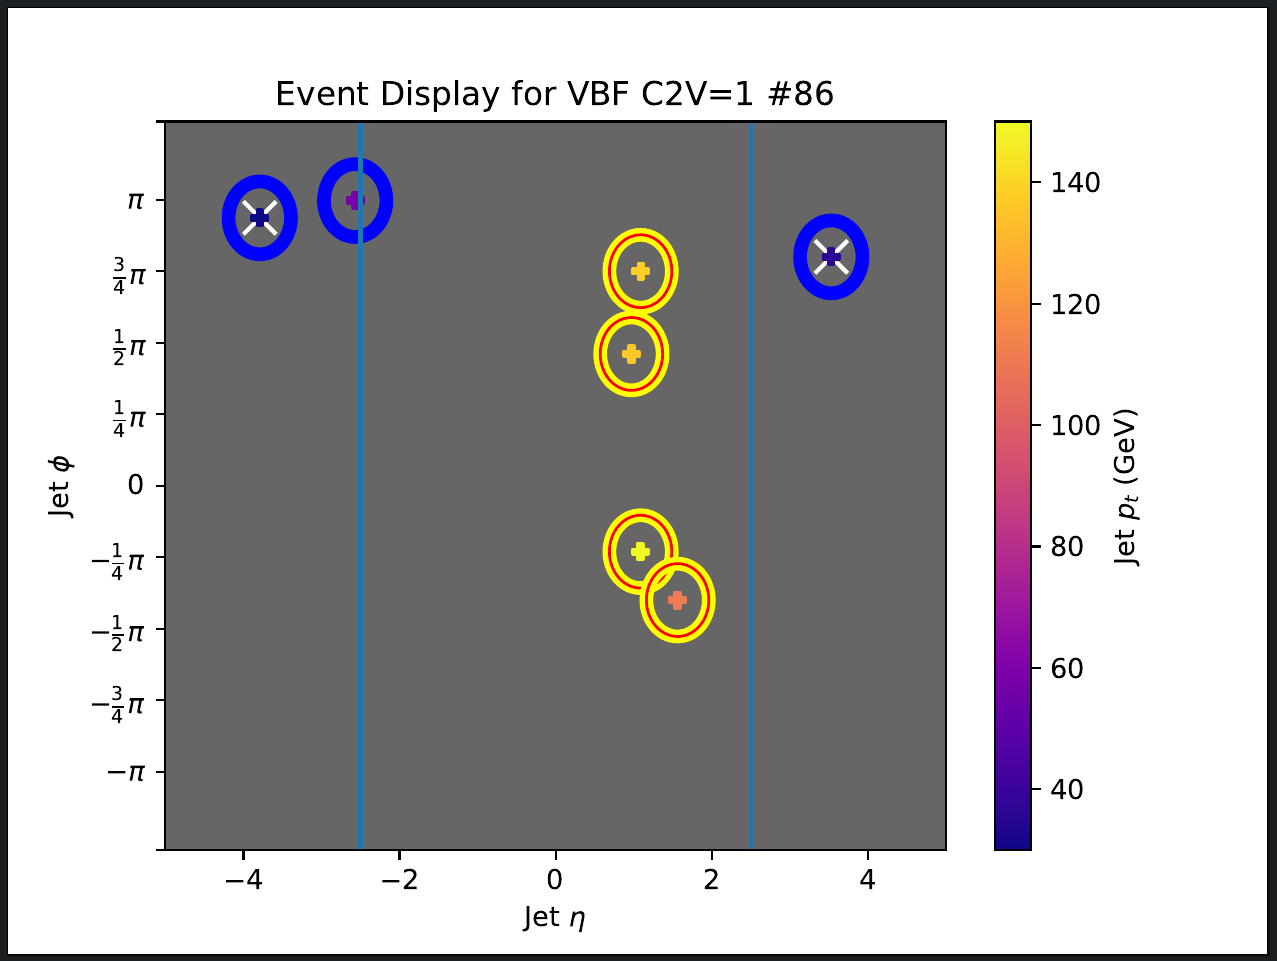
\includegraphics[width=\linewidth,height=0.9\textheight,keepaspectratio]{event_display}
            \caption{\tiny Rings indicate jets;
                Yellow ring => b-tagged;
                Blue ring w/ white cross => VBF initial-scatter jets;
                ``+" in center of rings => $p_T$;
                vertical lines denote "forward" vs "central" region.}
        \end{figure}
    \end{column} \end{columns}
}

\frame{
    \frametitle{Signal Modelling}
    \begin{columns} \begin{column}{0.5\textwidth}
        \begin{itemize}
            \item Signal modelled through MC event simulation
            \item Primarily generated at LO with MadGraph5
            \item Showering through Pythia8
            \item $t \bar t$ background simulated with Powheg-box
            \item Multi-jet backgrounds modelled using data
        \end{itemize}
    \end{column} \begin{column}{0.5\textwidth}
        {\small A number of different coupling values have been simulated to provide hypotheses at many points}

        \vspace{10mm}
        \begin{center} \resizebox{0.4\textheight}{!}{\begin{tabular}{ |l|l|l|l| }
            \hline
            \textbf {DSID} & \textbf {$\kappa_{2V}$} & \textbf {$\kappa_\lambda$} & \textbf {$\kappa_V$} \\
            \hline
                450044  &   1   & 1   & 1   \\ 
                450045  &   1   & 2   & 1   \\ 
                450046  &   2   & 1   & 1   \\ 
                450047  &   1.5 & 1   & 1   \\ 
                450049  &   0.5 & 1   & 1   \\ 
                450050  &   0   & 1   & 1   \\ 
                450052  &   1   & 0   & 1   \\ 
                450054  &   4   & 1   & 1   \\ 
                450055  &   1   & 10  & 1   \\ 
            \hline
        \end{tabular}} \end{center}
    \end{column} \end{columns}
    \vspace{5mm}

    \textbf{These coupling points do not by themselves constitute a comprehensive coverage of the full theoretical parameter space!}
}
